\subsubsection{Graphs}\label{subsec:graph_distribution}

Another prominent data structure is graphs, which can model 
social networks, citation networks, or knowledge graphs.
\citet{progcl_2022} propose an approach to mine negative samples for \ac{cl} on graphs called \progcl{}. 
As a motivation, the authors compare the similarity between the anchor and \acp{tn} 
to the similarity between the anchor and \acp{fn} 
across multiple datasets for both conventional \ac{cl} and \ac{gcl}.
The resulting distributions shown in \autoref{fig:sim_t_f_neg_image_graph} 
indicate that for \ac{gcl} the majority of highly similar negative samples are \acp{fn}, 
while for conventional \ac{cl} there seems to be no clear trend.
Moreover, the authors found that both the \ac{tn} and \ac{fn} distributions are best modeled by a beta mixture model %\acl{bmm} 
since it is able to fit the skewed empirical distribution.
The distribution is fitted using the \ac{em} algorithm on a subset of samples for a reduction of computational costs.

\begin{figure}%
    \centering
    \subfloat[\centering CIFAR-10 (Image)]
    {{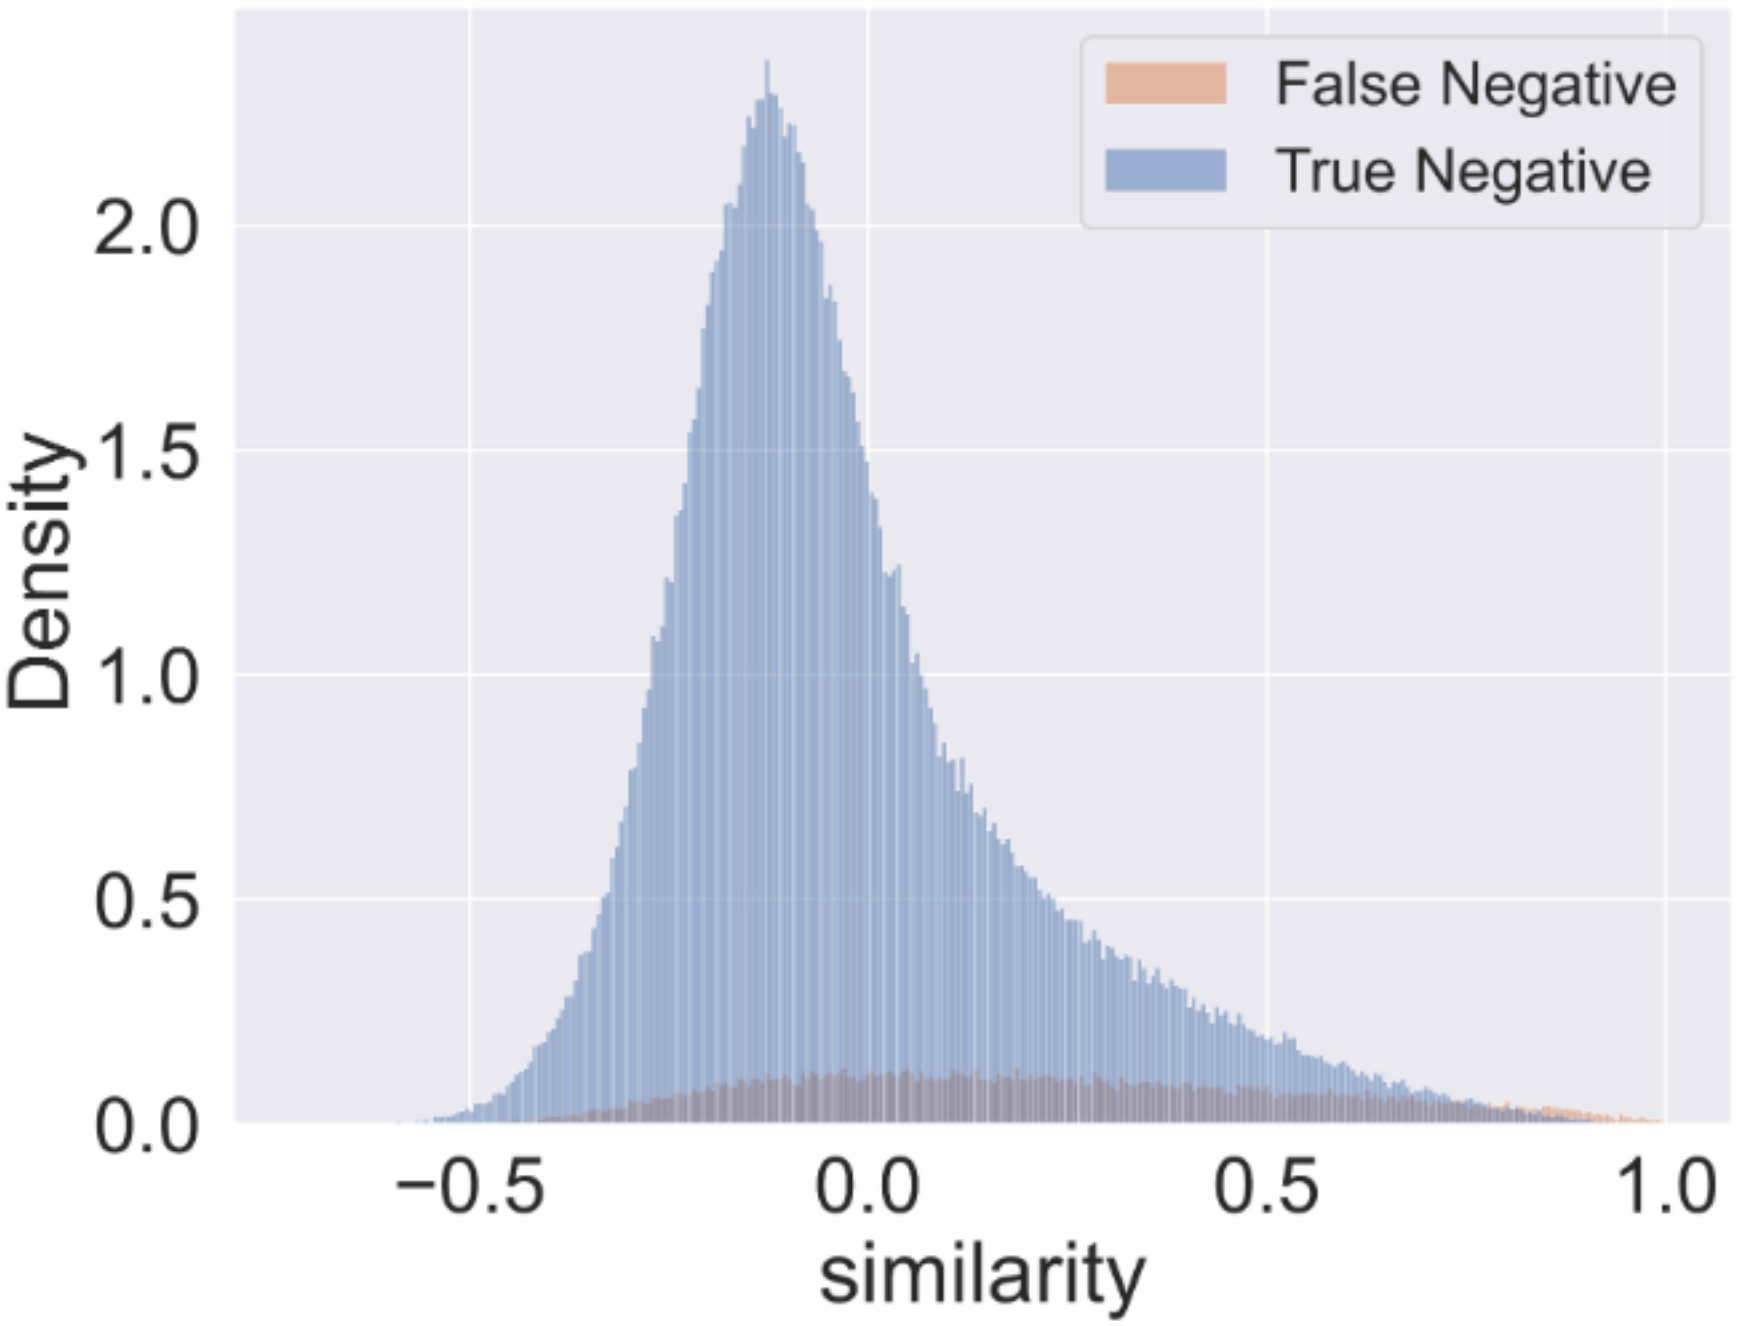
\includegraphics[width=4.8cm]{images/sim_negatives_image_data.png} }}%
    \qquad
    \subfloat[\centering Coauthor-CS (Graph). Most similar negative samples are \acp{fn}.]
    {{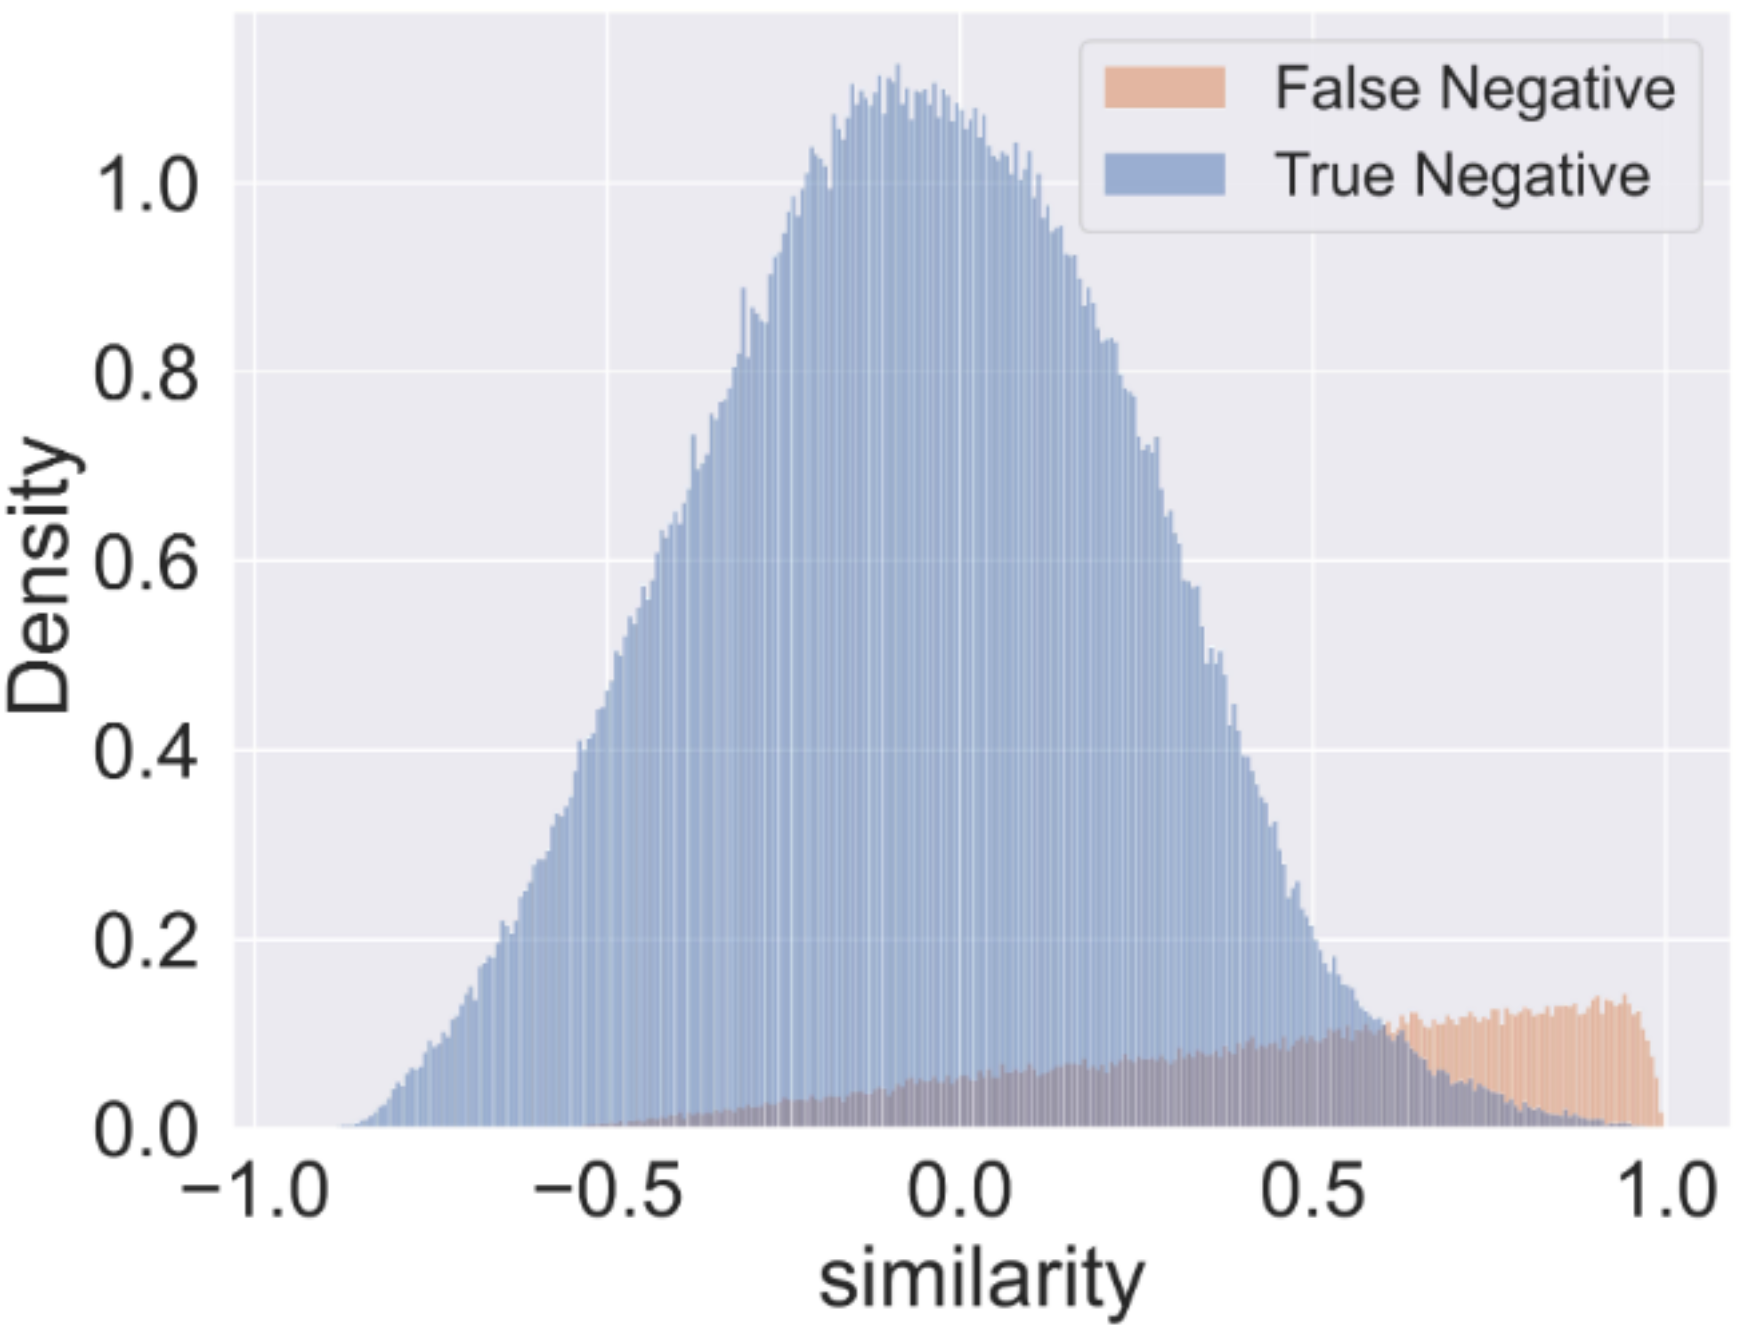
\includegraphics[width=5.2cm]{images/sim_negatives_graph_data.png} }}%
    \caption{Histogram of similarity between anchor and negative samples for \ac{cl} and \ac{gcl} from \citet{progcl_2022}.
    Blue denotes the empirical distribution of the \acp{tn}, while orange denotes \acp{fn}.}%
    \label{fig:sim_t_f_neg_image_graph}%
\end{figure}

% scheme 1: ProGCL-weight
Building on this observation, the authors propose incorporating both the probability of a sample being a \ac{tn} and 
the sample's similarity to the anchor, referred to as its hardness, into the negative sample selection process. 
The probability of a sample being a \ac{tn} is derived using Bayes' theorem in conjunction with 
the probability density function of a Beta Mixture Model, 
which is trained on a ground-truth dataset comprised of \acp{tn}.
It is important to note that the anchor is not a cluster center, 
but rather the sample from which augmentations are derived.

% scheme 2: ProGCL-mix (cf. MoCHi)